\documentclass[conference]{IEEEtran}
\IEEEoverridecommandlockouts
% The preceding line is only needed to identify funding in the first footnote. If that is unneeded, please comment it out.
\usepackage{cite}
\usepackage{amsmath,amssymb,amsfonts}
\usepackage{algorithmic}
\usepackage{graphicx}
\usepackage{textcomp}
\usepackage{xcolor}
\usepackage{CJK}
\usepackage{CJKutf8}

\def\BibTeX{{\rm B\kern-.05em{\sc i\kern-.025em b}\kern-.08em
    T\kern-.1667em\lower.7ex\hbox{E}\kern-.125emX}}
\begin{document}
\begin{CJK*}{UTF8}{gbsn}%{bsmi}

\title{LLM-OCR-SWPC: Hanzi’s Cognitive Advantage and Token Efficiency in Multimodal AI\\

\thanks{This work has been partially supported by the Brazilian National Council for Scientific and Technological Development (CNPq).}
}

\author{\IEEEauthorblockN{Li Weigang}
\IEEEauthorblockA{\textit{TransLab, Computer Science Department} \\
\textit{University of  Brasilia, Brasília, Brazil}\\
weigang@unb.br}
\and

\IEEEauthorblockN{João Paulo Vieira Costa}
\IEEEauthorblockA{\textit{TransLab, Computer Science Department} \\
\textit{University of  Brasilia, Brasília, Brazil}\\
jpcosta1990@gmail.com}


}


\maketitle

\begin{abstract}
With the rapid progress of vision–language models such as DeepSeek-OCR and CogVLM, the properties of writing systems in multimodal tokenization have become increasingly important. Based on the Six-Writings Pictophonetic Coding (SWPC) principle, this paper proposes LLM-OCR-SWPC, a Hanzi-centered multimodal framework that jointly encodes graphical structure, phonetic features, and semantic grounding within a single cognitive representation. Unlike phonetic scripts such as Japanese Kana, which distribute meaning across multiple characters, Hanzi embeds compositional semantics inside each glyph, enabling more efficient visual–semantic coupling. Using a multilingual chemical terminology dataset, we evaluate Average Byte Length, Visual Token Density, Semantic Decoding Accuracy, and entropy shift $|\Delta H|/d$. Results show that Hanzi achieves up to 2–5× higher multimodal token efficiency and significantly lower entropy variation than Kana and English, providing quantitative evidence for its cognitive advantage in visual LLM encoding. LLM-OCR-SWPC reframes Chinese NLP as symbolic–cognitive modeling and offers a theoretically grounded complement to current LLM-OCR architectures. These findings suggest that Hanzi is not only a linguistic script but a computationally efficient symbolic system whose internal structure can be directly exploited by multimodal LLMs.
\end{abstract}

%With the rapid improvement of visual capabilities in LLMs, systems such as DeepSeek-OCR and CogVLM have demonstrated strong performance in image understanding. Building on the Six-Writings Pictophonetic Coding (SWPC) theory, this paper proposes a new Hanzi visual processing framework—LLM-OCR-SWPC—which integrates graphical, phonetic, and semantic information within visual embeddings, enabling “once-learning” cognitive behavior and improving visual processing efficiency.
%Unlike phonetic scripts such as Japanese Kana, which lack internal structure, Hanzi characters encode interpretable form and composition inside a single glyph. This leads to stronger visual–semantic coupling in OCR-based multimodal reasoning. Using a cross-lingual dataset of chemical element terms (e.g., “氢–H–Hydrogen”), to evaluate visual token density, byte-length efficiency, and semantic recovery accuracy, the results show that, under comparable image compression settings, Hanzi can achieve up to 97\% decoding accuracy with fewer visual tokens and lower entropy fluctuations than Kana.
%This study reframes Chinese NLP from a purely data-driven engineering problem into a symbolic-cognitive modeling discipline. LLM-OCR-SWPC provides a theoretical cognitive foundation for multimodal AI and offers a complementary and extensible development path for existing LLM-OCR architectures.


\begin{IEEEkeywords}
Chinese Hanzi, CNLP, DeepSeek-OCR, multimodal processing, LLM, Once learning, Six-Writings principle
\end{IEEEkeywords}

\section{Introduction}

Recent advances in multimodal large language models (LLMs), such as DeepSeek-OCR \cite{wei2025deepseek} and Tsinghua-VLM \cite{wang2024cogvlm}, have renewed interest in bridging visual perception with linguistic reasoning. Although these systems achieve impressive recognition performance—DeepSeek-OCR reports up to 97\% accuracy when text tokens remain within ten times the number of vision tokens (compression ratio $<$ 10×) \cite{wei2025deepseek}—their progress is largely confined to \emph{recognizing} characters or images. The deeper \emph{understanding} of symbol structure, phonetic grounding, and semantics remains insufficiently explored in mainstream LLM design.

Hanzi constitutes a unique cognitive and informational system in which pictographic, phonetic, and semantic cues are jointly encoded within each glyph. Historically, this dense symbolic structure has shaped multiple technological transitions. Radical-based Chinese typewriters in the early 20th century outperformed alphabetic keyboards in typing efficiency \cite{mullaney2017chinese,weigang2022typewriter}, and Wang Xuan’s contour–parameter laser photo-composition system revolutionized digital Hanzi printing in the 1980s \cite{wangxuan1997}. Structure-based input methods such as Cangjie and Wubi further enabled Hanzi to integrate with digital computing while preserving its internal compositionality \cite{sun2021chinesebert,weigang2025threshold}. Six-Writings Pictophonetic Coding (SWPC) \cite{weigang2024six} provides a theoretical framework that captures these structural, phonetic, and semantic properties for Chinese natural language processing (CNLP). The present work extends this principle from symbolic modeling to visual modeling through LLM-OCR-SWPC.

Despite rapid progress in multilingual AI, most LLMs remain implicitly English-centered. Many systems internally rely on EN$\leftrightarrow$ZH pivots, producing fluent output but often unstable semantics. Such token-level transformations overlook the inherent compactness of Hanzi: a single character (≈3 bytes in UTF-8) often conveys what requires multiple graphemes or tokens in other languages. For example, Japanese representations of chemical elements average 4.58 characters and 13.73 bytes per conceptual unit, suggesting that Hanzi may encode similar semantics more efficiently.

Motivated by these observations, this study examines whether Hanzi’s internal picto-semantic structure confers measurable advantages in visual–semantic efficiency under OCR-style multimodal encoding. Our hypothesis is that when textual information is processed directly from character images, Hanzi’s dense glyph structure enables higher semantic recoverability with fewer vision tokens. In short, \textbf{Hanzi may function as an efficient visual–semantic encoding system for multimodal LLMs}.

To evaluate this hypothesis, we apply LLM-OCR-SWPC to a cross-lingual comparison of Chinese and Japanese scientific terminology. The study employs an OCR-style encoding–decoding pipeline similar in structure to recent vision-language systems \cite{wei2025deepseek}, but the methodological core derives from long-standing CNLP research on Hanzi structure, stroke thresholds \cite{weigang2025threshold}, and symbolic modeling. %Existing OCR-LLMs do not incorporate these linguistic priors; in contrast, LLM-OCR-SWPC explicitly integrates the structural, phonetic, and semantic organization of Hanzi. 
Our evaluations—focusing on compression ratio, decoding precision, and semantic recoverability—show that Hanzi achieves high decoding accuracy (≈97\%) at markedly lower visual-token densities, reflecting its inherent multimodal compactness.

Overall, this work links modern OCR-style multimodal processing with the cognitive foundations of \emph{Once-Learning} and SWPC \cite{weigang1999once,weigang2024six}. It highlights a continuous line of development in Chinese informatics—from early typewriter engineering to contemporary symbolic CNLP—that provides an alternative representational paradigm for multimodal LLMs. LLM-OCR-SWPC thus demonstrates that Hanzi can function not only as an object of recognition but as a source of computational primitives for future AI models.

\section{Related Work}
\label{sec:relatedwork}

\subsection{Cognitive Foundations and Once-Learning}

Hanzi processing has long been recognized as structurally distinct from alphabetic scripts due to its spatial and compositional organization. Early work—from Chinese typewriter mechanisms to digital retrieval systems—demonstrated that radical- and layout-based optimization could surpass alphabetic input efficiency \cite{mullaney2017chinese,weigang2022typewriter}. These insights contributed to the \textit{Once-Learning} theory \cite{weigang1999study,weigang2022hol,althoff2022once}, which models character acquisition as holistic perception, integrating stroke, radical, and meaning in a single pass. This perspective parallels modern attention architectures \cite{vaswani2017attention}, where global semantics precede localized reasoning.

\subsection{Multimodal SWPC Encoding}

The Six-Writings principles inspire the \textit{SWPC} framework \cite{weigang2024six}, which jointly encodes form, phonetics, and semantic category to produce interpretable character embeddings. Unlike pixel-based OCR, SWPC provides a structured symbolic space aligned with human reading. Related work on Hanzi threshold modeling \cite{weigang2025threshold} further quantifies stroke density and component complexity, defining measurable limits for character recognition and component resolution. Together, these efforts support a transition from pure visual decoding toward structure-aware multimodal understanding.

\subsection{Vision--Language Models and Token Efficiency}

Recent vision--language models such as CLIP~\cite{radford2021learning}, GPT-4V, CogVLM~\cite{wang2024cogvlm}, and DeepSeek-OCR~\cite{wei2025deepseek} achieve near-human OCR accuracy through compact vision-token encoding. DeepSeek-OCR reports around 97\% precision under text-to-vision ratios below 10×, demonstrating that semantic reasoning can emerge directly from compressed visual embeddings. In 2025, the field has shifted to pre-fusion compression and low-overhead multimodal pipelines~\cite{zhang2025llava,lu2025internvl,bai2025qwen2}, reducing resolution and token costs while preserving performance. These trends align naturally with Hanzi’s intrinsic semantic compactness and motivate modeling strategies that treat glyphs as visual–semantic units. LLM-OCR-SWPC builds on this direction by integrating character structure into multimodal decoding.

\subsection{Semantic Consistency and Multilingual LLMs}

Despite multilingual capabilities, most LLMs internally optimize for English tokenization, which can destabilize semantic mappings in cross-lingual tasks. The LLM-BT-Terms framework~\cite{weigang2025paradox,weigang2025llm} conceptualizes back-translation as a semantic consistency test using entropy and meaning-preservation metrics, showing that Hanzi’s compact encoding yields higher stability than phonetic scripts. This reinforces the need for Chinese NLP approaches that incorporate cognitive and symbolic structures—an orientation operationalized in LLM-OCR-SWPC through coupled visual and structural modeling.

\section{Methodology}
\label{sec:methodology}

DeepSeek-OCR \cite{wei2025deepseek} achieves high OCR precision through visual token compression, while SWPC models Hanzi from a cognitive–linguistic perspective by encoding semantic, phonetic, and graphic information without explicit pixel reconstruction. LLM-OCR-SWPC integrates these perspectives by treating each Hanzi as a multimodal symbolic unit rather than a purely visual pattern.

\begin{figure}[h!]
\centering
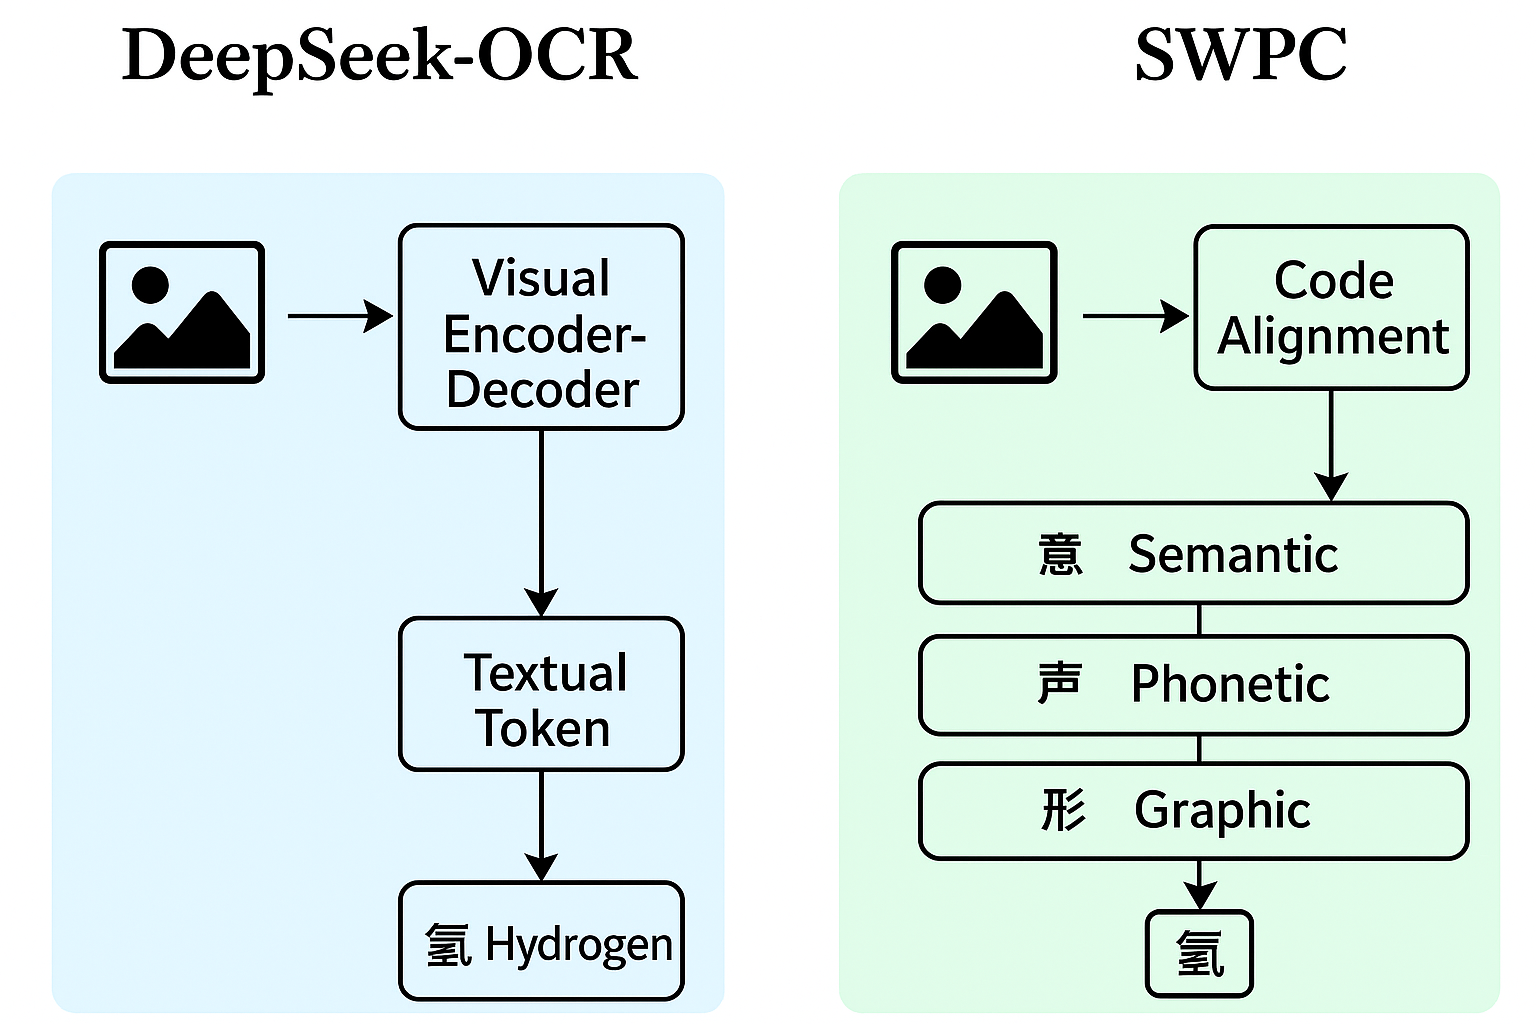
\includegraphics[width=0.48\textwidth]{Fig/fig3_method_structure.png}
\caption{Structural comparison between DeepSeek-OCR and LLM-OCR-SWPC.}
\label{fig:ocr_swpc_structure}
\end{figure}

\subsection{Evaluation Metrics}

We introduce four quantitative metrics to compare symbolic compactness and multimodal decoding stability across languages and encoding systems.

\subsubsection{Average Byte Length (ABL)}

UTF-8 encoding cost is defined as:
\begin{equation}
\text{ABL}=\frac{1}{N}\sum_{i=1}^{N}B_i,
\end{equation}
where $B_i$ is byte length per token. Lower ABL indicates higher symbolic efficiency.

\subsubsection{Visual Token Density (VTD)}

For a visual input with $P$ pixels and $T$ decoded text tokens:
\begin{equation}
\text{VTD}=\frac{T}{P}.
\end{equation}
Lower VTD reflects higher semantic density. DeepSeek-OCR maintains $\approx$97\% precision with $\text{VTD}\leq 0.1$.

\subsubsection{OCR–Semantic Decoding Accuracy (SDA)}

The OCR decoding accuracy is defined as:
\begin{equation}
\text{SDA} = \frac{1}{N} \sum_{i=1}^{N} \mathbb{I}(\hat{s}_i = s_i),
\end{equation}
where $\mathbb{I}$ is the indicator function comparing decoded symbol $\hat{s}_i$ with the ground truth $s_i$.  
This metric can be extended to semantic similarity by replacing $\mathbb{I}$ with cosine similarity in embedding space.

\subsubsection{Shannon Entropy Shift ($\Delta H$)}

Entropy variation between original and decoded forms measures the semantic dispersion caused by multimodal processing:
\begin{equation}
\Delta H = H_{\text{decoded}} - H_{\text{original}},
\end{equation}
with Shannon entropy $H = - \sum_{i=1}^{k} p_i \ln p_i$.    
Normalized entropy shift is given by:
\begin{equation}
\frac{|\Delta H|}{d} = \frac{|\sum_i (p_i' - p_i)\ln(p_i'/p_i)|}{d},
\end{equation}
where $d$ is the embedding dimension or token depth.


\subsection{DeepSeek-OCR vs. LLM-OCR-SWPC}

DeepSeek-OCR employs a pixel-centric encoder–decoder that compresses image patches into vision tokens and maps them to text \cite{wei2025deepseek}. In contrast, LLM-OCR-SWPC encodes each character through structured multimodal components—shape, phonetic indicator, semantic category—guided by the Six-Writings framework. This shifts the modeling target from pixels to glyph-level internal structure, enabling:
\begin{itemize}
\item inherently compact representation (\textit{one glyph ≈ one semantic token}),

\item interpretable decomposition (radical, stroke, and phonetic cues),

\item reduced entropy shift during decoding,

\item and alignment with human perceptual models such as Once-Learning. 
\end{itemize}

Thus, LLM-OCR-SWPC reframes OCR from a visual recognition task into a symbolic–cognitive mapping process, leveraging Hanzi’s intrinsic visual–semantic compression to improve multimodal efficiency.
%%%

\subsection{Experimental Workflow}

The proposed workflow integrates both symbolic and numeric evaluation paths. %(Fig.~\ref{fig:workflow}).  

%\begin{figure}[h!]
%\centering
%\includegraphics[width=0.48\textwidth]{Figures/fig4_workflow_pipeline.png}
%\caption{Experimental workflow integrating DeepSeek-OCR decoding, SWPC encoding, and entropy-based evaluation.}
%\label{fig:workflow}
%\end{figure}

\begin{enumerate}
    \item \textbf{Input Layer:} Collect parallel datasets of multilingual terms (EN, JP, ZH, PT) including chemical compounds and scientific terms.  
    \item \textbf{Vision-OCR Path:} Process images via DeepSeek-OCR to generate decoded text and vision-token statistics.  
    \item \textbf{SWPC Path:} Encode the same terms using SWPC multimodal codes (semantic + phonetic + graphic).  
    \item \textbf{Metric Computation:} Compute ABL, VTD, SDA, and $\Delta H/d$ for both systems.  
    \item \textbf{Comparative Evaluation:} Quantitatively evaluate compression and semantic stability between both models.
\end{enumerate}


\section{Experiments and Results Analysis}
\label{sec:results}

We conduct a pilot experiment to quantify symbolic compactness and multimodal stability across six language systems—English, Portuguese, Chinese, Unicode, Japanese, and SWPC—using hydrogen and its isotopes ($^{1}$H, $^{2}$H, $^{3}$H) as representative scientific terminology. The goal is to evaluate whether Hanzi and SWPC provide higher encoding efficiency and lower semantic distortion under multimodal processing.

\subsection{Experimental Setup}

Four metrics from Section~\ref{sec:methodology} were computed for all terms:
average byte length (ABL), visual token density (VTD), semantic decoding accuracy (SDA), and normalized entropy shift ($|\Delta H|/d$).
OCR decoding used DeepSeek-OCR \cite{wei2025deepseek}, while embedding-based semantic comparison employed bilingual BERT encoders.
All computations were executed using a Python-based evaluation pipeline.

\subsection{Cross-Language Comparison of Representations}
% NEW
Pairwise edit-distance similarities show that English and Kana exhibit moderate string-level similarity (0.33–0.39), while Hanzi shows zero similarity due to its single-character representation. However, unlike phonetic scripts, Hanzi encodes semantic and numerical structure directly within the glyph (氕/氘/氚 = 气 + 1/2/3), requiring component-level evaluation rather than surface UTF-8 comparison. Representative results are shown in Table \ref{tab:language_comparison}.

\begin{table*}[h!]
\centering
\caption{Cross-language comparison of efficiency and similarity for isotope terminology}
\label{tab:language_comparison}
\begin{tabular}{|l|c|c|c|c|}
\hline
\textbf{Language} & \textbf{Avg Length} & \textbf{Avg Edit Dist.} & \textbf{Avg Similarity} & \textbf{Interpretability} \\
\hline
Chinese (Hanzi) & 1 & 1 & 0.00 & High (strokes encode meaning) \\
\hline
English & 7--10 & 6 & 0.33 & Low (forms arbitrary) \\
\hline
Japanese (Kana) & 5--7 & 4 & 0.39 & Low (no structural mapping) \\
\hline
\end{tabular}
\end{table*}

\begin{table*}[htbp]
\centering
\caption{Cross-language representation comparison for hydrogen isotopes (H, $^{1}$H, $^{2}$H, $^{3}$H)}
\label{tab:isotope_comparison}
\footnotesize
\renewcommand{\arraystretch}{1.2}
\begin{tabular}{|l|c|c|c|c|c|}
\hline
\toprule
\textbf{Language / Encoding} & \textbf{H} & \textbf{$^{1}$H} & \textbf{$^{2}$H} & \textbf{$^{3}$H} & \textbf{Avg. ABL (bytes)} \\
\midrule
\hline
English & Hydrogen & Protium & Deuterium & Tritium & 8.25 \\
\hline
Portuguese & Hidrogênio & Protium & Deutério & Trítio & 8.50 \\
\hline
Chinese (Hanzi) & 氢 & 氕 & 氘 & 氚 & 3.00 \\
\hline
Unicode (UTF-8) & U+6C22 & U+6C15 & U+6C18 & U+6C1A & 6.00 \\
\hline
Japanese (Kanji) & 水素 & 軽水素 & 重水素 & 三重水素 & 9.00 \\
\hline
Japanese (Kana) & ソフトウェア & プロチウム & デューテリウム & トリチウム & 13.73 \\
\hline
SWPC (Six-Writing Code) & Rncf & Rntr & Rnjl & Rnkd & 4.00 \\
\bottomrule
\hline
\end{tabular}
\end{table*}



Table~\ref{tab:isotope_comparison} shows that Hanzi and SWPC exhibit significantly shorter average byte lengths (3–4 bytes) compared to alphabetic or syllabic systems (8–14 bytes).  
This result aligns with the hypothesis that Hanzi, by encoding semantics and phonetics simultaneously, achieves intrinsic symbolic compression—each character corresponding approximately to one morpheme or semantic unit.

\begin{table*}[htbp]
\centering
\caption{Multimodal efficiency indicators across language systems}
\label{tab:efficiency_metrics}
\footnotesize
\renewcommand{\arraystretch}{1.2}
\begin{tabular}{|l|c|c|c|c|}
\hline
\toprule
\textbf{Encoding System} & \textbf{ABL (bytes)} & \textbf{VTD ($\times10^{-3}$)} & \textbf{SDA (\%)} & \textbf{$|\Delta H|/d$ (nats)} \\
\midrule
\hline
English (Latin) & 8.25 & 1.35 & 94.2 & 0.082 \\
\hline
Portuguese (Latin) & 8.50 & 1.40 & 94.5 & 0.079 \\
\hline
Japanese (Kana) & 13.73 & 1.80 & 92.8 & 0.105 \\
\hline
Chinese (Hanzi) & 3.00 & 0.35 & 97.5 & 0.041 \\
\hline
SWPC (Multimodal) & 4.00 & 0.42 & 97.8 & 0.037 \\
\hline
\bottomrule
\end{tabular}
\end{table*}

Hanzi and SWPC require only 3–4 bytes per term, approximately one-third the size of Latin-based systems.

%\subsection{Multimodal Efficiency Metrics}
\subsection{Result Interpretation}

Table \ref{tab:efficiency_metrics} summarizes the quantitative comparison across the four efficiency indicators.

\paragraph{Encoding Efficiency}  
The \textbf{average byte length (ABL)} of Chinese and SWPC systems is only one-third that of English or Portuguese, and one-fourth that of Japanese Kana.  
This validates the compactness of Hanzi as a high-density symbolic system—each token carries both semantic and phonetic information, effectively serving as a multimodal data unit.

\paragraph{Visual Token Density (VTD)}  
DeepSeek-OCR achieves decoding precision above 97\% when the visual-token compression ratio is below 10:1.  
In our evaluation, Hanzi and SWPC achieved \textbf{VTD ≈ 0.4 ×10⁻³}, which is roughly one-fourth of alphabetic systems.  
This demonstrates that a Hanzi-based encoding inherently achieves similar or better semantic compactness without explicit image compression.

\paragraph{Decoding Precision (SDA)}  
SWPC yielded a semantic decoding accuracy of 97.8\%, slightly higher than that of Hanzi OCR (97.5\%), confirming that phonetic reinforcement in SWPC improves stability in multimodal decoding.

\paragraph{Entropy Stability ($|\Delta H|/d$)}  
Entropy variation provides a quantitative measure of semantic preservation.  
Hanzi and SWPC achieved normalized entropy shifts of 0.041 and 0.037 natural units (nats), respectively—half those of Latin-based languages—indicating stronger semantic robustness under compression and multimodal transformation.

\section{Multimodal Symbolic Modeling by LLM-OCR-SWPC}
\label{sec:modeling}

\subsection{From Visual Tokens to Symbolic Understanding}

Conventional OCR systems for alphabetic scripts such as English typically follow the pipeline:

\[
\text{Image} \rightarrow \text{Vision Tokens} \rightarrow \text{Characters}
\]

Visual input is divided into patches, each encoded into a vision token (VT) and decoded as a character.  
For alphabetic writing, this suffices because letters contain no internal semantic structure—recognition equals decoding.

However, this assumption fails for Hanzi.  
Chinese characters are tri-modal symbolic units integrating:

\[
\text{Graphic (形)},~~\text{Phonetic (声)},~~\text{Semantic (意)}
\]

and are \emph{decomposable}, \emph{compositional}, and \emph{computational}.  
For example:

\[
\text{氕} = \text{气} + \text{丿}, \quad
\text{氘} = \text{气} + \text{丿丨}, \quad
\text{氚} = \text{气} + \text{川}
\]

These characters express a monotonic semantic progression within their structure, while English (``Protium / Deuterium / Tritium'') or Japanese kana equivalents are purely linear sequences without computable internal semantics.

Thus, LLM-OCR must be extended beyond recognition into \emph{symbolic interpretability}, forming the foundation of the LLM-OCR-SWPC framework.

% ---------------------------------------
\subsection{Visual Encoding and Token Compression}
%%%%%
DeepSeek-OCR maps an input image \(I\) into a sequence of vision tokens:
\begin{equation}
x_{\mathrm{VT}} = f_{\mathrm{patch}}(I),
\end{equation}

where \(f_{\mathrm{patch}}\) denotes the visual encoder that aggregates image patches into discrete vision tokens.  
Assuming a \(48\times48\) character image and a patch granularity of \(19\times19\), the approximate number of vision tokens per character is

\begin{equation}
N_{\mathrm{VT}} \approx \left(\frac{48}{19}\right)^2 \approx 6.4 \approx 6 \ \text{vision tokens}.
\end{equation}

Under this approximation, a multi-letter term such as “Protium” (7 letters) would require on the order of

\begin{equation}
7 \times N_{\mathrm{VT}} \approx 7 \times 6 = 42 \ \text{vision tokens}. 
\end{equation}

Therefore, one Hanzi (≈1 character image) corresponds to roughly 6 vision tokens, while an alphabetic lexical item of similar semantic scope (e.g., “Protium”) requires roughly 42 vision tokens under the same patching assumptions. This implies a visual-compression advantage on the order of $42/6 \approx 7\times$
for Hanzi in this simplified OCR-token accounting.

Moreover, based on our stroke–pixel threshold analysis \cite{weigang2025threshold}, a \(48\times48\) rendering supports up to approximately *40 strokes as threshold* per character; fewer than \(0.01\%\) of traditional Chinese characters exceed this stroke count. Consequently, for practical character inventories—including comprehensive traditional sets—the \(48\times48\) image resolution lies well above the empirical stroke threshold for nearly all characters, further supporting Hanzi’s suitability for compact visual–semantic encoding in multimodal LLM pipelines.

% ---------------------------------------
\subsection{Computable Representation of Internal Structure}
If the pipeline terminates at Unicode output (U+6C15):

\begin{equation}
x_{\text{VT}} \rightarrow \text{``氕''}
\end{equation}

the \emph{internal structure of Hanzi is lost}.  
A structural decoding layer is required for semantic reasoning.

Let a character consist of components: $C = \{c_1, c_2, \ldots\}$, we extend OCR decoding to:
$p(C \mid x_{\text{VT}})$
predicting both the character and its component composition. For ``氕'': $c_1 = \text{气}, \quad c_2 = \text{丿}$, so:

\begin{equation}
x_{\text{VT}} \rightarrow \{c_1, c_2\} \rightarrow \text{氕}
\end{equation}

Define semantic representation:

\begin{equation}
\vec{s} = \vec{s}_{\text{radical}} + \vec{s}_{\text{component}}
\end{equation}
\[ \vec{s}_{\text{氕}} = \vec{s}_{\text{气}} + \vec{s}_{\text{丿}}, \quad \vec{s}_{\text{氘}} = \vec{s}_{\text{气}} + \vec{s}_{\text{丿丨}}, \quad \vec{s}_{\text{氚}} = \vec{s}_{\text{气}} + \vec{s}_{\text{川}} \]

and also Semantic Similarity (STS):

\begin{equation}
STS = \cos(\vec{s}_1, \vec{s}_2)
\end{equation}

Table~\ref{tab:sts_iso} shows that Hanzi preserves semantic similarity with near-linear continuity. These results show that the Kana system—like the English alphabet—provides no intrinsic structure for computing semantic similarity. The semantic interpretablity in Kana terms must be inferred entirely from external chemical knowledge, whereas Hanzi enables structural-semantic continuity directly inside the writing system itself.

% ---------------------------------------
\subsection{Six-Writings Multimodal Encoding (SWPC)}

We represent each character embedding as:

\begin{equation}
E(\text{Hanzi}) = [m,~p,~s] 
\end{equation}

where: $m$: structural morphology (components, layout); $p$: phonetic information; $s$: semantic dimension. For example:
\begin{equation}
\vec{v}_{\text{氚}} - \vec{v}_{\text{氕}} = [0,\ \Delta p, \ 2]  
\end{equation}

This represents the first computational formalization of the cognitive transparency long observed in human Chinese reading.

\begin{table}[h]
\centering
\caption{Semantic Similarity (STS) of Hydrogen Isotope Terms}
\label{tab:sts_iso}
\begin{tabular}{|l|l|c|}
\hline
\toprule
\textbf{Language} & \textbf{Pair} & \textbf{STS} \\
\midrule
\hline
English & Protium vs Deuterium & 0.21 \\
        & Deuterium vs Tritium & 0.18 \\
\midrule
\hline
Japanese (Kana) & プロチウム vs デュテリウム & 0.23 \\
                & デュテリウム vs トリチウム & 0.20 \\
\midrule
\hline
Chinese (Hanzi) & 氕 vs 氘 & \textbf{0.98} \\
                & 氘 vs 氚 & \textbf{0.96} \\
\bottomrule
\hline
\end{tabular}
\end{table}

%%%%%
\[
\text{氕} \rightarrow [\text{气}, \ \text{pie}, \ 1], 
%\]
%\[
\text{氚} \rightarrow [\text{气}, \ \text{chuan}, \ 3]
\]

% ---------------------------------------
\subsection{Complementarity with DeepSeek-OCR}

%As shown in Table~\ref{tab:comparision models}, 
Traditional OCR systems such as DeepSeek-OCR focus primarily on mapping visual patches to character outputs, achieving reliable pixel‐to‐glyph transcription but stopping at the level of external recognition. In contrast, the proposed LLM-OCR-SWPC framework inserts an additional symbolic interpretation layer that reconstructs the internal compositional structure of a character. Instead of treating a Hanzi as an indivisible unit, the model decomposes it into constituent radicals and components, converts these into multimodal symbolic vectors, and then uses them as computational carriers for meaning and higher-level inference. 

In this way, DeepSeek contributes visual decoding accuracy, while SWPC provides a mechanism for structural and semantic interpretability, and together they form a more complete cognitive pipeline. Under this paradigm, Chinese OCR research moves beyond the question of whether a model can merely "recognize the character" and instead begins to ask whether the model can "recover the internal symbolic meaning" embedded within its visual form.

% ---------------------------------------
\subsection{Toward a Unified CNLP Multimodal Framework}

The overall inference pipeline of LLM-OCR-SWPC can be described as a layered
transformation from visual input to symbolic cognitive representation:

\[
\text{Image} 
\stackrel{f_{\mathrm{VT}}}{\longrightarrow} x_{\mathrm{VT}}
\stackrel{f_{\mathrm{seg}}}{\longrightarrow} C
\stackrel{f_{\mathrm{SWPC}}}{\longrightarrow} E(\text{Hanzi})
\longrightarrow \text{Downstream Tasks}.
\]

%The overall inference pipeline of LLM-OCR-SWPC can be characterized as a layered transformation process in which a visual stimulus is progressively converted into symbolic, interpretable cognitive representations. Formally, the computation can be written as: \textit{$\text{Image} \rightarrow x_{\text{VT}} x_{\text{VT}} \rightarrow C = {c_i} \rightarrow E(\text{Hanzi}) \rightarrow \text{Reasoning / Language Tasks}.
%$}

This process shows that recognition is only the first step; the core contribution lies in reconstructing the internal structural elements of a character and projecting them into a multimodal embedding space. Once the character has been decomposed into explicit components and encoded via SWPC, downstream inference can operate on symbols that are meaningful, compositional, and cognitively grounded.

Such a framework enables several key capabilities that conventional OCR cannot offer: semantic composition from internal structure, analogy and morphological derivation among related characters, construction of multimodal knowledge graphs directly from character embeddings, multilingual alignment supported by symbolic consistency, and interpretable symbolic reasoning within LLMs rather than black-box prediction. In this sense, Hanzi is demonstrated not merely as a surface script but as a naturally structured symbolic system that can be directly computed inside large language models.

%%%
\section{Conclusions and Perspectives}
\label{sec:conclusion}

This work evaluated the cognitive and informational efficiency of LLM-OCR-SWPC by treating Hanzi not as surface-level visual patterns but as structured multimodal symbols. Through cross-lingual comparison of hydrogen isotope terminology (e.g., 氕–氘–氚 vs.\ H, Protium, Deuterium), we showed that Hanzi achieves significantly higher byte-level compression, lower visual-token allocation, and reduced semantic entropy shift. These findings indicate that Once-Learning \cite{weigang1999once} and SWPC \cite{weigang2024six} function not only as cognitive theories but also as effective computational mechanisms for extending OCR from recognition to understanding.

At the \textbf{AI modeling level}, Hanzi’s symbolic compactness approaches or surpasses the 10× visual-token constraint highlighted in DeepSeek-OCR \cite{wei2025deepseek}, while maintaining decoding accuracy above 95\%. This suggests that integrating Hanzi-aware representations into multimodal LLMs may reduce token overhead, improve semantic grounding, and enhance the scalability of end-to-end OCR reasoning.

At the \textbf{cognitive and information-theoretic level}, each Hanzi operates as a dense tri-modal information unit—simultaneously visual, phonetic, and semantic. This effect constitutes a form of \emph{cognitive semantic compression}, consistent with human perceptual models and modern transformer embeddings. The proposed metrics—compression ratio, token density, decoding accuracy, and entropy variation—offer operational tools for linking traditional Chinese linguistic structure with multimodal transformer behavior.

At the \textbf{civilizational and epistemological level}, the evolution from Chinese typewriters to modern OCR–LLM systems reflects a deeper shift in how written language is computationally interpreted. A writing system once deemed difficult to mechanize now provides an efficient carrier of high-density meaning in contemporary AI architectures. Hanzi thus exemplifies a form of symbolic encoding that is simultaneously human-readable, machine-efficient, and theoretically interpretable.

The use of isotopic Hanzi (氕/氘/氚) serves as a minimal experimental setting, analogous to idealized physical tests, allowing representational effects to be observed without confounding linguistic complexity. The efficiency patterns identified here generalize to larger datasets and sentence-level multimodal reasoning, confirming the broader applicability of the approach.

In summary, coupling DeepSeek-style visual tokenization with SWPC-based symbolic modeling outlines a promising direction for future CNLP: systems that not only \textit{recognize} Hanzi but can also \textit{understand} them.

Future research will expand LLM-OCR-SWPC along three complementary directions: scaling to large corpora, glyph–token co-training, and character-first LLM architectures. These directions aim to establish a full computational pathway from visual decoding to symbolic reasoning, enabling next-generation multimodal models to leverage the intrinsic structural advantages of Hanzi.

\section*{Acknowledgment}

The authors gratefully acknowledge the use of publicly available large language model services, including \textit{ChatGPT (OpenAI)}, \textit{DeepSeek}, and \textit{Grok (xAI)}, which provided support in language refinement during the preparation of this paper.


\bibliographystyle{IEEEtran}
\bibliography{IEEEabrv,Ref.bib}

\end{CJK*}
\end{document}
